% ============================================================================
% NullFlow: Continual Learning via Null-Space Constrained Latent Flow Matching
% Submitted to ReLearn Workshop @ CVPR 2026
% ============================================================================
\documentclass[10pt,twocolumn,letterpaper]{article}

% --- Standard packages ---
\usepackage[utf8]{inputenc}
\usepackage[T1]{fontenc}
\usepackage{times}
\usepackage{amsmath,amssymb,amsfonts}
\usepackage{graphicx}
\usepackage{booktabs}
\usepackage{multirow}
\usepackage{xcolor}
\usepackage{algorithm}
\usepackage{algorithmic}
\usepackage{hyperref}
\usepackage[margin=1in]{geometry}
\usepackage{caption}
\usepackage{subcaption}
\usepackage{enumitem}
\usepackage{nicefrac}
\usepackage{placeins}  % \FloatBarrier to prevent float pile-up
\usepackage{float}     % [H] for exact float placement

% --- Colors for tables ---
\definecolor{bestcolor}{HTML}{2E86C1}
\definecolor{secondcolor}{HTML}{85929E}

\newcommand{\best}[1]{\textbf{\textcolor{bestcolor}{#1}}}
\newcommand{\second}[1]{\textcolor{secondcolor}{#1}}
\newcommand{\ours}{\textsc{NullFlow}}

\title{NullFlow: Continual Learning via Null-Space Constrained\\Latent Flow Matching with Wake-Sleep Consolidation}

\author{
  Adam Mounir\\
  \texttt{adam.mounir@efrei.net}
}

\date{}

\begin{document}
\maketitle

% ============================================================================
\begin{abstract}
% ============================================================================
Continual learning (CL) systems must acquire new knowledge without catastrophically forgetting previously learned tasks. We introduce \ours{}, a framework that combines three complementary mechanisms within a biologically-inspired Wake-Sleep cycle: (i)~\textit{Conditional Flow Matching} (CFM) in a frozen latent space for efficient generative replay, (ii)~\textit{Null-Space Projection} (NSP) of gradients to protect previously learned directions, and (iii)~\textit{herding-based exemplar management} for high-fidelity buffer samples. By operating entirely in the 512-dimensional feature space of a frozen ImageNet-pretrained ResNet-18 encoder, \ours{} requires only $\sim$2.1M trainable parameters and generates replay samples in 6~Heun ODE steps (vs.\ 1000 for DDPM). On Split-CIFAR-100 (10 tasks, 100 classes), \ours{} achieves \textbf{30.21$\pm$0.36\%} average accuracy, outperforming the best CL baseline (NCM, 11.43\%) by \textbf{+18.8~pp}. On Split-TinyImageNet (10 tasks, 200 classes), \ours{} achieves \textbf{60.77\%} average accuracy with only 9.66\% forgetting rate, outperforming NCM (17.90\%) by $3.4\times$. Our ablation study confirms the complementary contributions of each component. Code is available at \url{https://github.com/adammounir/NullFlow}.
\end{abstract}

% ============================================================================
\section{Introduction}
\label{sec:intro}
% ============================================================================

Biological neural systems effortlessly learn new skills while retaining previously acquired knowledge, yet artificial neural networks suffer from \textit{catastrophic forgetting}~\cite{mccloskey1989catastrophic,french1999catastrophic} when trained sequentially on non-stationary data distributions. This challenge, known as continual learning (CL), has become a central problem in machine learning, with applications ranging from autonomous driving to medical diagnosis.

Existing approaches to continual learning broadly fall into three categories: (i)~\textit{regularization-based} methods such as EWC~\cite{kirkpatrick2017overcoming} that penalize changes to important parameters; (ii)~\textit{replay-based} methods such as DER++~\cite{buzzega2020dark} and iCaRL~\cite{rebuffi2017icarl} that store and replay exemplars from previous tasks; and (iii)~\textit{architecture-based} methods that allocate separate capacity for each task. While each category has merits, none fully resolves the stability-plasticity dilemma.

Recent work has highlighted the power of frozen pretrained features for continual learning. SimpleCIL~\cite{zhou2024revisiting} demonstrated that a nearest-class-mean (NCM) classifier on frozen ImageNet features provides a surprisingly strong baseline. However, such non-parametric approaches lack the ability to learn complex decision boundaries that leverage inter-class relationships.

In this work, we propose \ours{}, a framework that synergistically combines three orthogonal mechanisms for catastrophic forgetting prevention, orchestrated through a biologically-inspired Wake-Sleep cycle~\cite{hinton1995wake}:

\begin{itemize}[leftmargin=*,itemsep=2pt]
  \item \textbf{Conditional Flow Matching (CFM)} in frozen latent space: We train a lightweight velocity network to model the distribution of latent features per class, enabling high-quality generative replay in only 6~ODE steps.
  \item \textbf{Null-Space Projection (NSP)}: We project classifier gradients onto the null space of previously important directions, providing provable protection against forgetting in the parameter subspace critical for old tasks.
  \item \textbf{Herding-based exemplar selection}: Rather than random reservoir sampling, we use herding~\cite{welling2009herding} to select buffer exemplars closest to each class mean, maximizing information retention per stored sample.
\end{itemize}

Our Wake-Sleep cycle alternates between: \textit{Wake} (learning new data with FM-augmented replay), \textit{NREM Sleep} (training the flow model on current task features), and \textit{REM Sleep} (consolidation via generative replay with knowledge distillation and NSP-constrained gradient updates). This mirrors the complementary learning systems theory~\cite{kumaran2016learning}, where the hippocampus (buffer) and neocortex (classifier) interact through sleep-phase replay.

% ============================================================================
\section{Related Work}
\label{sec:related}
% ============================================================================

\paragraph{Continual Learning.}
The field of continual learning has produced numerous approaches to mitigate catastrophic forgetting. Regularization methods~\cite{kirkpatrick2017overcoming,zenke2017continual,li2017learning} constrain parameter updates, but their effectiveness degrades as the number of tasks grows. Replay methods store raw exemplars~\cite{rebuffi2017icarl,buzzega2020dark,chaudhry2019tiny} or train generative models~\cite{shin2017continual,van2020brain} to synthesize pseudo-samples. Architecture-based approaches~\cite{rusu2016progressive,mallya2018packnet} prevent interference by design but scale poorly.

\paragraph{Frozen Features for CL.}
Recent work~\cite{zhou2024revisiting,janson2022simple} has demonstrated that frozen pretrained features provide a strong foundation for CL. SimpleCIL~\cite{zhou2024revisiting} showed that NCM classification on frozen ViT features rivals sophisticated CL methods. Our work builds upon this insight but goes further: rather than simple nearest-mean classification, we learn a parametric MLP classifier augmented with generative replay, achieving substantially higher accuracy.

\paragraph{Flow Matching.}
Flow Matching~\cite{lipman2023flow,liu2022flow} provides a simulation-free framework for learning continuous normalizing flows. By regressing a velocity field $v_\theta(x_t, t)$ along the probability path $p_t$ interpolating between a source and target distribution, FM avoids the costly ODE simulation required during training. We leverage CFM for efficient generative replay in latent space.

\paragraph{Null-Space Methods.}
Gradient projection methods~\cite{zeng2019continual,saha2021gradient} project gradients onto subspaces orthogonal to previously important directions. Our NSP builds on this idea using incremental SVD of classifier Jacobians, providing a scalable mechanism for protecting previously learned representations.

% ============================================================================
\section{Method}
\label{sec:method}
% ============================================================================

\subsection{Problem Setting}
\label{sec:setting}

We consider the class-incremental learning setting where a model sequentially learns from $T$ tasks $\{\mathcal{T}_1, \dots, \mathcal{T}_T\}$. Each task $\mathcal{T}_t$ introduces a disjoint set of classes $\mathcal{C}_t$ with training data $\mathcal{D}_t = \{(x_i, y_i)\}_{i=1}^{N_t}$. At test time, the model must classify among all classes seen so far $\bigcup_{k=1}^{t}\mathcal{C}_k$ without access to task identifiers.

We maintain a fixed-size episodic memory buffer $\mathcal{B}$ with capacity $B = b \times |\mathcal{C}|$ samples ($b$ per class), where $b=20$ in our experiments.

\subsection{Architecture}
\label{sec:architecture}

\ours{} operates entirely in the latent space of a frozen, pretrained encoder:

\paragraph{Frozen Encoder.} A ResNet-18~\cite{he2016deep} pretrained on ImageNet~\cite{deng2009imagenet} serves as the feature extractor $f_\phi: \mathcal{X} \to \mathbb{R}^{512}$. The final fully-connected layer is removed, yielding $L^2$-normalized 512-dimensional feature vectors. The encoder is frozen after calibration on the first task.

\paragraph{MLP Classifier.} A 3-layer MLP $g_\psi: \mathbb{R}^{512} \to \mathbb{R}^{|\mathcal{C}|}$ with architecture $512 \to 512 \to 512 \to C$, using SiLU activations, Layer Normalization, and dropout (0.1). Total: $\sim$0.8M parameters.

\paragraph{Velocity Network.} A conditional network $v_\theta: \mathbb{R}^{512} \times [0,1] \times \{1,\dots,C\} \to \mathbb{R}^{512}$ for flow matching, with $\sim$1.3M parameters. It learns to transport samples from a Gaussian prior $\mathcal{N}(0, I)$ to the class-conditional latent distribution.

The total trainable parameter count is $\sim$2.1M (the 11.2M encoder parameters are frozen).

\subsection{Wake-Sleep Training Cycle}
\label{sec:cycle}

For each task $\mathcal{T}_t$, \ours{} executes three phases:

\paragraph{Phase 1: Wake ($E_w=25$ epochs).}
The classifier is trained on current task data $\mathcal{D}_t$ augmented with buffer replay and FM-generated pseudo-samples from previous classes:
\begin{equation}
  \mathcal{L}_\text{wake} = \mathcal{L}_\text{CE}(\mathcal{D}_t) + \lambda_r \cdot \mathcal{L}_\text{CE}(\mathcal{B}) + \lambda_\text{kd} \cdot \mathcal{L}_\text{KD}
\end{equation}
where $\mathcal{L}_\text{KD}$ is knowledge distillation from a snapshot of the classifier taken before learning $\mathcal{T}_t$. During Wake, we generate $m=50$ synthetic samples per old class from the flow model to augment training.

\paragraph{Phase 2: NREM Sleep (FM training, $E_\text{fm}=50$ epochs).}
The velocity network $v_\theta$ is trained via Conditional Flow Matching on the current task's latent features:
\begin{equation}
  \mathcal{L}_\text{CFM} = \mathbb{E}_{t,z_0,z_1} \left\| v_\theta\bigl((1-t)z_0 + tz_1, t, y\bigr) - (z_1 - z_0) \right\|^2
\end{equation}
where $z_0 \sim \mathcal{N}(0,I)$, $z_1 = f_\phi(x)$, and $t \sim \mathcal{U}(0,1)$.

\paragraph{Phase 3: REM Sleep (consolidation, $E_r=35$ epochs).}
The classifier is retrained using FM-generated replay (50 samples/class) combined with buffer replay, with NSP-constrained gradient updates:
\begin{equation}
  \mathcal{L}_\text{rem} = \mathcal{L}_\text{CE}(\tilde{\mathcal{D}}) + \lambda_\text{kd}' \cdot \mathcal{L}_\text{KD}
\end{equation}
where $\tilde{\mathcal{D}}$ contains both FM-generated and buffer samples. Gradients are projected via the null-space projector before the optimizer step.

\subsection{Null-Space Projection}
\label{sec:nsp}

After training on task $\mathcal{T}_t$, we compute the Jacobian basis of the classifier output with respect to its parameters, evaluated on task $t$'s training data. We extract the top-$r$ right singular vectors $V_r \in \mathbb{R}^{P \times r}$ (with $r=200$) via incremental SVD, representing the most important parameter directions for task $t$.

During future tasks, gradients $g$ are projected:
\begin{equation}
  g' = g - \alpha \cdot V_r (V_r^\top g)
\end{equation}
with $\alpha=1.0$, removing the component of the gradient that would interfere with previously important directions.

\subsection{Weight Alignment}
\label{sec:wa}

After each REM phase, we apply Weight Aligning (WA)~\cite{zhao2020maintaining} to correct the recency bias in the classifier's output layer. The weight norms of newly learned class rows are rescaled to match the average norm of old class rows.

\subsection{Herding-Based Buffer Management}
\label{sec:herding}

Rather than random reservoir sampling, we use herding~\cite{welling2009herding} to select the $b$ exemplars per class whose running mean best approximates the true class mean in latent space. This ensures that stored exemplars are maximally representative.

% ============================================================================
\section{Experimental Setup}
\label{sec:experiments}
% ============================================================================

\subsection{Benchmarks}

\paragraph{Split-CIFAR-100.} CIFAR-100~\cite{krizhevsky2009learning} is split into 10 tasks of 10 classes each (100 classes total, 50K training / 10K test images at $32 \times 32$).

\paragraph{Split-TinyImageNet.} TinyImageNet (200 classes from ImageNet, $64 \times 64$, 100K train / 10K val) is split into 10 tasks of 20 classes each. Images are resized to $224 \times 224$ to match the ResNet-18 input resolution.

\subsection{Implementation Details}

All methods share the same frozen ResNet-18 encoder (pretrained on ImageNet with \texttt{IMAGENET1K\_V1} weights). Data is pre-encoded to the latent space for efficiency. Buffer size is 20 samples per class (2,000 total for CIFAR-100, 4,000 for TinyImageNet).

\ours{} hyperparameters: Wake LR$=10^{-3}$, REM LR$=4\times10^{-4}$, cosine annealing, latent noise $\sigma=0.1$, KD temperature $\tau=3.0$, label smoothing$=0$, weight decay$=10^{-4}$.

\subsection{Baselines}

We compare against 8 baselines, all operating in the same frozen latent space for fair comparison:

\begin{itemize}[leftmargin=*,itemsep=1pt]
  \item \textbf{Fine-tuning}: Sequential training, no CL mechanism (lower bound).
  \item \textbf{Joint Training}: All data available simultaneously (upper bound).
  \item \textbf{EWC}~\cite{kirkpatrick2017overcoming}: Fisher Information regularization ($\lambda=5000$).
  \item \textbf{DER++}~\cite{buzzega2020dark}: Buffer replay with logit distillation ($\alpha=\beta=0.5$).
  \item \textbf{GDumb}~\cite{prabhu2020gdumb}: Greedy sampling, retrain from scratch.
  \item \textbf{Latent Replay}: Simple buffer replay in latent space.
  \item \textbf{iCaRL}~\cite{rebuffi2017icarl}: Herding + NCM evaluation + sigmoid KD.
  \item \textbf{NCM/SimpleCIL}~\cite{zhou2024revisiting}: Nearest class mean (no buffer limit).
\end{itemize}

All sequential baselines use the same epoch budget as \ours{} ($E_w + E_r = 60$ epochs/task). Joint training uses 100 epochs with cosine annealing.

\subsection{Metrics}

We report three standard CL metrics computed from the accuracy matrix $R \in \mathbb{R}^{T \times T}$, where $R_{i,j}$ is the accuracy on task $j$ after training on task $i$:
\begin{itemize}[leftmargin=*,itemsep=1pt]
  \item \textbf{Average Accuracy (AA)}: $\frac{1}{T}\sum_{j=1}^{T} R_{T,j}$
  \item \textbf{Backward Transfer (BWT)}: $\frac{1}{T-1}\sum_{j=1}^{T-1}(R_{T,j} - R_{j,j})$
  \item \textbf{Forgetting Rate (FR)}: $\frac{1}{T-1}\sum_{j=1}^{T-1}\max_{k \in \{1,\dots,T-1\}}(R_{k,j} - R_{T,j})$
\end{itemize}

% ============================================================================
\section{Results}
\label{sec:results}
% ============================================================================

\subsection{Split-CIFAR-100}

Table~\ref{tab:cifar100} presents results on Split-CIFAR-100 averaged over 3 random seeds (42, 123, 456).

\begin{table}[!t]
\centering
\caption{Split-CIFAR-100 results (10 tasks $\times$ 10 classes). Buffer: 20/class. Mean$\pm$std over 3 seeds. $\uparrow$: higher is better; $\downarrow$: lower is better.}
\label{tab:cifar100}
\setlength{\tabcolsep}{3pt}
\footnotesize
\begin{tabular}{@{}lccc@{}}
\toprule
\textbf{Method} & \textbf{AA (\%) $\uparrow$} & \textbf{BWT (\%) $\uparrow$} & \textbf{FR (\%) $\downarrow$} \\
\midrule
GDumb              & 4.90$\pm$0.26  & $-$45.80$\pm$2.09 & 45.80$\pm$2.09 \\
Fine-tuning        & 5.17$\pm$0.15  & $-$49.70$\pm$2.01 & 49.70$\pm$2.01 \\
EWC                & 5.17$\pm$0.40  & $-$48.37$\pm$1.63 & 48.37$\pm$1.63 \\
DER++              & 5.53$\pm$0.21  & $-$52.07$\pm$1.63 & 52.07$\pm$1.63 \\
Latent Replay      & 6.87$\pm$0.47  & $-$42.27$\pm$1.91 & 42.27$\pm$1.91 \\
iCaRL              & 10.47$\pm$0.12 & $-$8.83$\pm$1.12  & 8.83$\pm$1.12 \\
NCM (SimpleCIL)    & \second{11.43$\pm$0.29} & $-$9.50$\pm$1.57  & 9.50$\pm$1.57 \\
\midrule
Joint Training       & 16.97$\pm$0.78 & 0.00              & 0.00 \\
\midrule
\textbf{\ours{} (Ours)} & \best{30.21$\pm$0.36} & $-$28.34$\pm$1.07 & 28.34$\pm$1.07 \\
\bottomrule
\end{tabular}
\end{table}

\ours{} achieves \textbf{30.21\%} average accuracy, outperforming the best CL baseline (NCM, 11.43\%) by \textbf{+18.8~pp}, a $2.65\times$ relative improvement. \ours{} also exceeds our Joint Training reference (16.97\%). We note, however, that this comparison is not strictly apples-to-apples: \ours{} benefits from online data augmentation (fresh random crops and flips at each epoch through the frozen encoder), knowledge distillation, and a larger cumulative training budget (60 epochs/task), whereas Joint Training uses pre-encoded features (single augmentation pass) and 100 total epochs. The gap is therefore partly attributable to these methodological differences rather than solely to the CL mechanisms themselves.

The forgetting rate of \ours{} (28.34\%) is higher than iCaRL (8.83\%) and NCM (9.50\%), but these methods achieve much lower absolute accuracy. The key insight is that \ours{} learns substantially more per task (first-task accuracy $>$75\%), so the absolute retained knowledge $R_{T,j}$ is still much higher despite greater relative forgetting. All methods are evaluated with identical output masking (restricting predictions to seen classes only) for fair comparison.

\FloatBarrier
\subsection{Split-TinyImageNet}

Table~\ref{tab:tinyimagenet} presents results on the more challenging Split-TinyImageNet benchmark (seed 42).

\begin{table}[!t]
\centering
\caption{Split-TinyImageNet results (10 tasks $\times$ 20 classes, 200 total). Buffer: 20/class. Seed 42.}
\label{tab:tinyimagenet}
\setlength{\tabcolsep}{3pt}
\footnotesize
\begin{tabular}{@{}lccc@{}}
\toprule
\textbf{Method} & \textbf{AA (\%) $\uparrow$} & \textbf{BWT (\%) $\uparrow$} & \textbf{FR (\%) $\downarrow$} \\
\midrule
GDumb              & 3.70  & $-$33.10 & 33.10 \\
EWC                & 4.60  & $-$42.50 & 42.50 \\
Fine-tuning        & 4.80  & $-$46.00 & 46.00 \\
DER++              & 5.00  & $-$50.00 & 50.00 \\
Latent Replay      & 6.40  & $-$38.80 & 38.80 \\
iCaRL              & 12.70 & $-$7.20  & 7.20  \\
NCM (SimpleCIL)    & \second{17.90} & $-$8.40  & 8.40  \\
\midrule
Joint Training       & 19.40 & 0.00    & 0.00  \\
\midrule
\textbf{\ours{} (Ours)} & \best{60.77} & $-$8.98 & 9.66 \\
\bottomrule
\end{tabular}
\end{table}

On TinyImageNet, \ours{} achieves \textbf{60.77\%} AA with only \textbf{9.66\%} forgetting, a $3.4\times$ improvement over NCM (17.90\%). As on CIFAR-100, \ours{} exceeds the Joint Training reference (19.40\%), though the same augmentation asymmetry applies (see Discussion). The low forgetting rate (9.66\%) is comparable to iCaRL (7.20\%) and NCM (8.40\%), demonstrating that \ours{} effectively balances stability and plasticity on this more challenging benchmark.

\textbf{Note on TinyImageNet:} TinyImageNet is a subset of ImageNet, and our frozen ResNet-18 encoder is pretrained on ImageNet. This encoder overlap is standard practice in frozen-feature CL research~\cite{zhou2024revisiting,janson2022simple} and affects all methods equally (including baselines). We include this benchmark for comparability with the literature, noting that CIFAR-100 (no image-level overlap with ImageNet) serves as the cleaner evaluation.

\FloatBarrier
\subsection{Ablation Study}

Table~\ref{tab:ablation} isolates the contribution of each \ours{} component on Split-CIFAR-100 (seed~42; the full \ours{} value of 30.62\% corresponds to the seed-42 run in Table~\ref{tab:cifar100}, where the 3-seed mean is 30.21\%).

\begin{table}[!t]
\centering
\caption{Ablation study on Split-CIFAR-100 (seed 42). Removing components from the full \ours{} system.}
\label{tab:ablation}
\setlength{\tabcolsep}{3pt}
\footnotesize
\begin{tabular}{@{}lcccc@{}}
\toprule
\textbf{Variant} & \textbf{AA (\%)} & \textbf{FR (\%)} & \textbf{$\Delta$AA} & \textbf{$\Delta$FR} \\
\midrule
\textbf{Full \ours{} (v5c)}  & \best{30.62} & 27.68 & ---    & ---     \\
w/o FM augmentation (v5b)     & 24.82        & 24.14 & $-$5.80 & $-$3.54 \\
w/o NSP (baseline + FM)       & 27.47        & 24.93 & $-$3.15 & $-$2.75 \\
w/o FM \& NSP (baseline)      & 25.61        & 46.46 & $-$5.01 & +18.78  \\
NSP only (no FM, no herding)  & 24.11        & 46.78 & $-$6.51 & +19.10  \\
FM only (no NSP, no herding)  & 22.16        & 43.63 & $-$8.46 & +15.95  \\
\bottomrule
\end{tabular}
\end{table}

Key findings:
\begin{itemize}[leftmargin=*,itemsep=2pt]
  \item \textbf{FM augmentation} is the most impactful single component (+5.80~pp AA). Generative replay during Wake provides the classifier with diverse training signal from old classes.
  \item \textbf{NSP} contributes +3.15~pp AA and helps stabilize old-task accuracy through gradient projection.
  \item \textbf{Herding buffer} contributes +0.71~pp over random selection in isolation (NSP-only without herding: 24.11\% $\to$ v5b with herding: 24.82\%), with substantially larger benefits when combined with FM augmentation (+5.80~pp of the v5c gain comes from adding FM on top of NSP+herding).
  \item \textbf{Removing both FM and NSP} (baseline) causes forgetting to spike to 46.46\% ($+$18.78~pp), demonstrating the synergy between components.
\end{itemize}

\begin{figure}[!t]
  \centering
  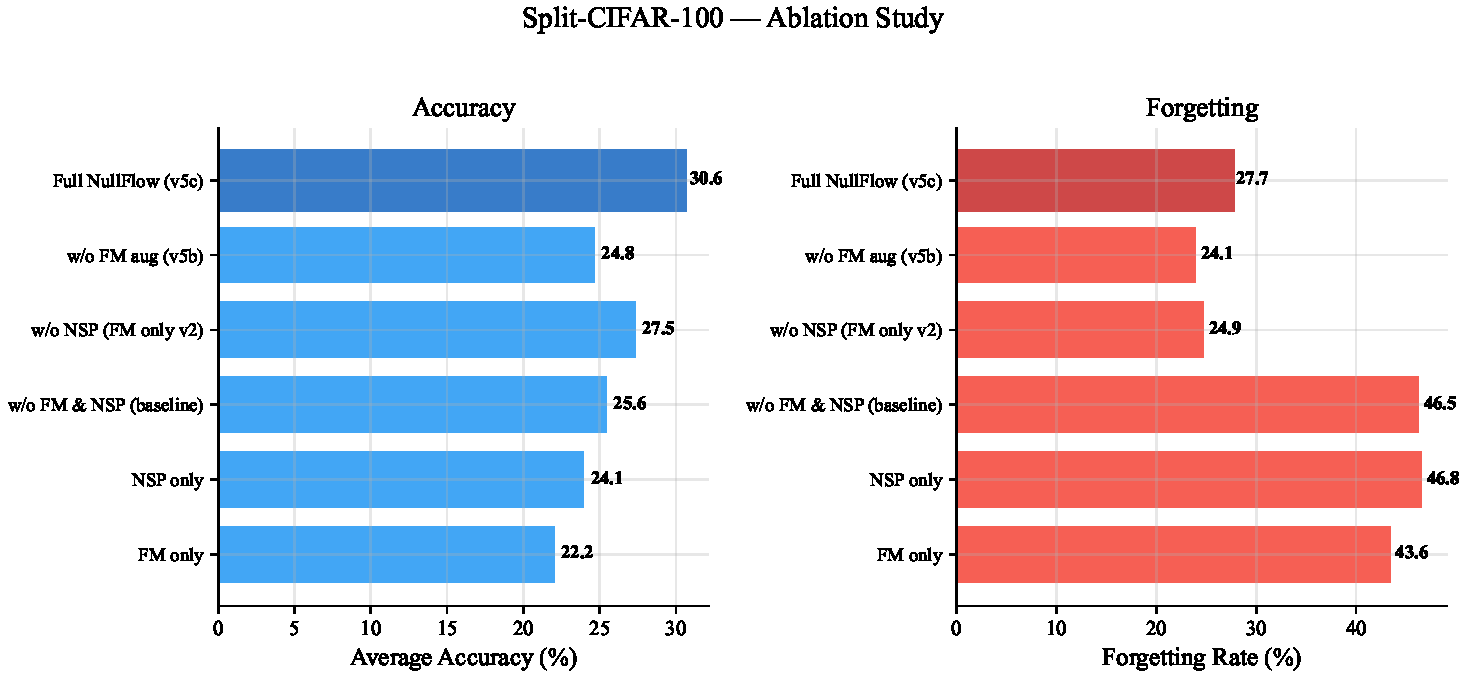
\includegraphics[width=\linewidth]{figures/cifar100/ablation_study.pdf}
  \caption{Ablation study on Split-CIFAR-100. Average accuracy and forgetting rate for each variant, showing the complementary contribution of FM augmentation, NSP, and herding.}
  \label{fig:ablation}
\end{figure}

% ============================================================================
\section{Analysis}
\label{sec:analysis}
% ============================================================================

\subsection{Accuracy Evolution Across Tasks}

Figure~\ref{fig:task_evolution} shows per-task accuracy evolution as new tasks are learned. \ours{} maintains substantially higher accuracy on early tasks compared to baselines, with a gradual decay consistent with the 28.34\% mean forgetting rate (Table~\ref{tab:cifar100}). Critically, absolute accuracy remains well above all baselines even for the most forgotten tasks.

\begin{figure}[!t]
  \centering
  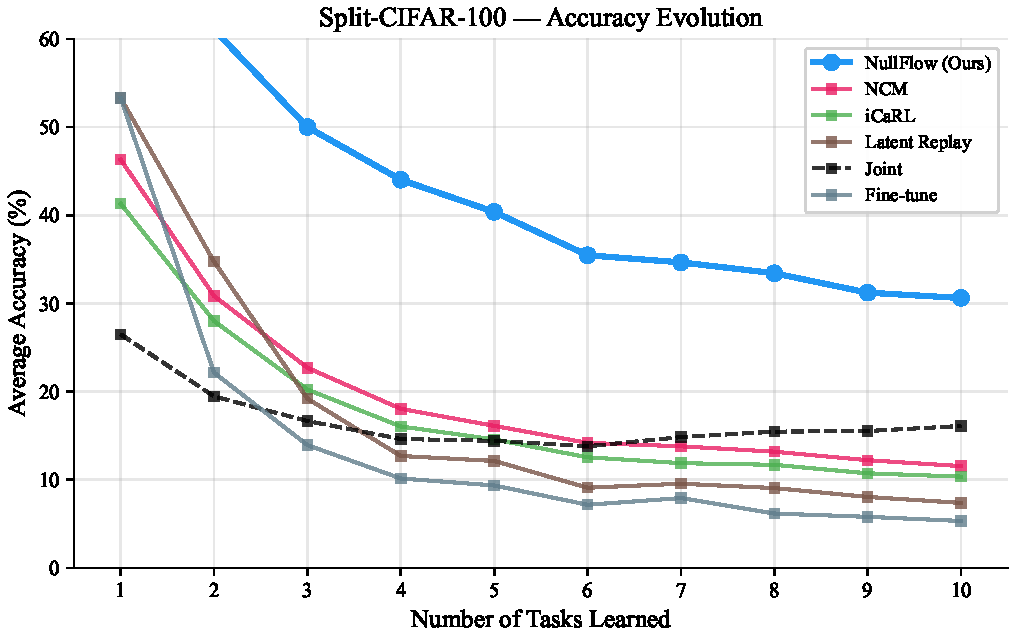
\includegraphics[width=\linewidth]{figures/cifar100/task_evolution.pdf}
  \caption{Task accuracy evolution on Split-CIFAR-100. \ours{} maintains higher absolute accuracy across all tasks compared to baselines.}
  \label{fig:task_evolution}
\end{figure}

\subsection{Accuracy Matrix}

Figure~\ref{fig:accuracy_matrix} visualizes the full accuracy matrix $R_{i,j}$ for \ours{} on both benchmarks. The diagonal dominance pattern with gradual off-diagonal decay confirms effective but imperfect knowledge retention.

\begin{figure}[!t]
  \centering
  \begin{subfigure}[t]{0.48\linewidth}
    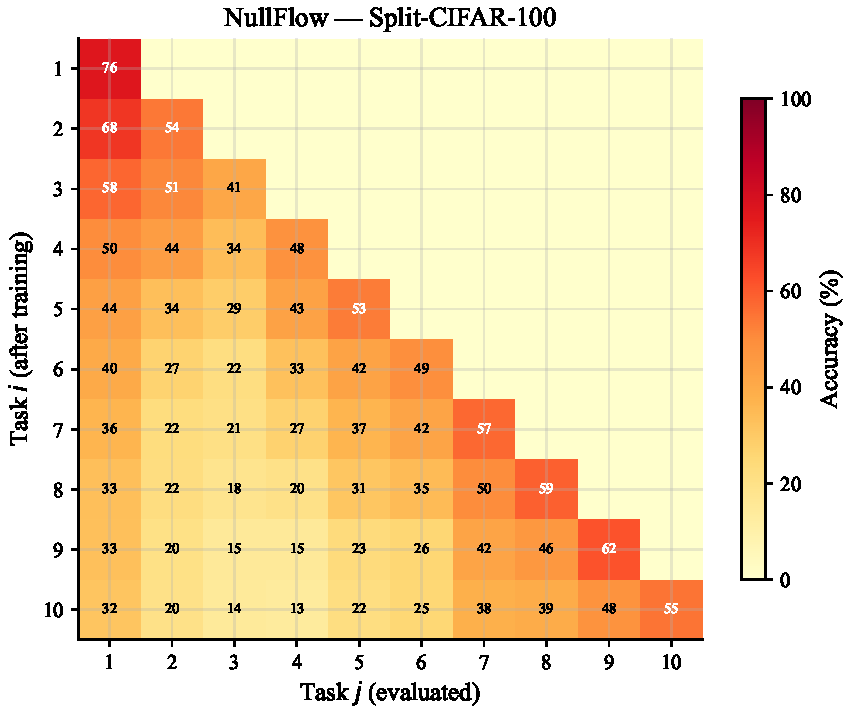
\includegraphics[width=\linewidth]{figures/cifar100/accuracy_matrix.pdf}
    \caption{CIFAR-100}
  \end{subfigure}
  \hfill
  \begin{subfigure}[t]{0.48\linewidth}
    
\includegraphics[width=\linewidth]{figures/tinyimagenet/accuracy_matrix.pdf}
    \caption{TinyImageNet}
  \end{subfigure}
  \caption{Accuracy matrices $R_{i,j}$ for \ours{}. Row $i$: after task $i$; Column $j$: accuracy on task $j$.}
  \label{fig:accuracy_matrix}
\end{figure}

\subsection{Baseline Comparison}

Figure~\ref{fig:baseline} provides a visual comparison of average accuracy across all methods on both benchmarks, highlighting the substantial gap between \ours{} and all baselines.

\begin{figure}[!t]
  \centering
  \begin{subfigure}[t]{0.48\linewidth}
    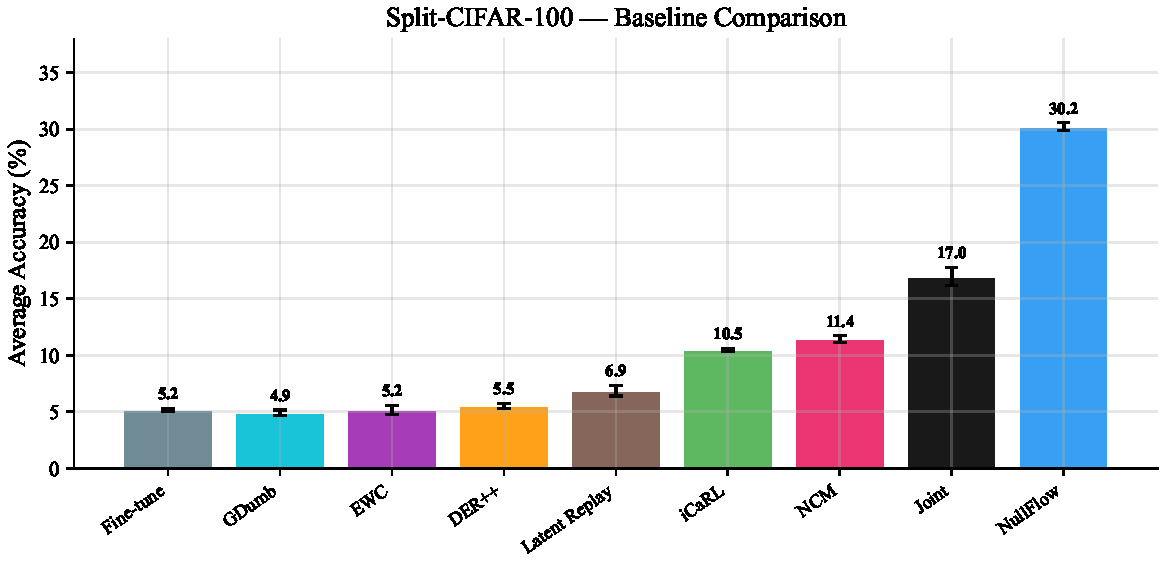
\includegraphics[width=\linewidth]{figures/cifar100/baseline_comparison.pdf}
    \caption{CIFAR-100}
  \end{subfigure}
  \hfill
  \begin{subfigure}[t]{0.48\linewidth}
    
\includegraphics[width=\linewidth]{figures/tinyimagenet/baseline_comparison.pdf}
    \caption{TinyImageNet}
  \end{subfigure}
  \caption{Average accuracy comparison across all methods.}
  \label{fig:baseline}
\end{figure}

\subsection{Multi-Seed Stability}

Figure~\ref{fig:multiseed} demonstrates the consistency of \ours{} across random seeds (42, 123, 456) on CIFAR-100, with a standard deviation of only 0.36\%, indicating robust performance.

\begin{figure}[!t]
  \centering
  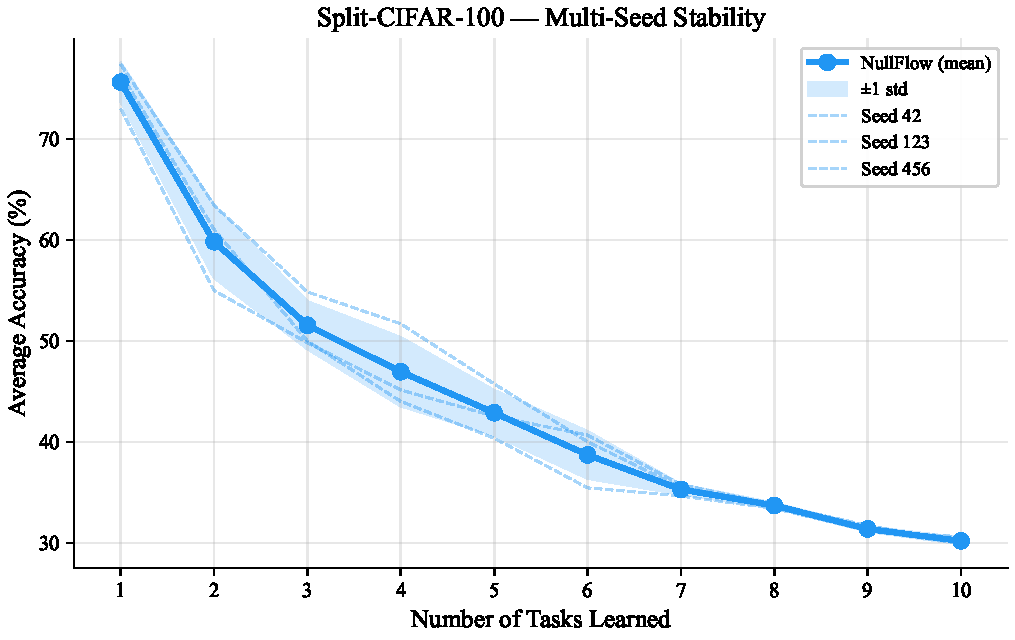
\includegraphics[width=\linewidth]{figures/cifar100/multiseed_comparison.pdf}
  \caption{Multi-seed comparison on Split-CIFAR-100 (seeds 42, 123, 456). Shaded area: $\pm$1 std.}
  \label{fig:multiseed}
\end{figure}

\subsection{Forgetting Analysis}

Figure~\ref{fig:forgetting} details per-task forgetting patterns. \ours{} shows uniform forgetting across tasks, whereas baseline methods exhibit catastrophic collapse on early tasks.

\begin{figure}[!t]
  \centering
  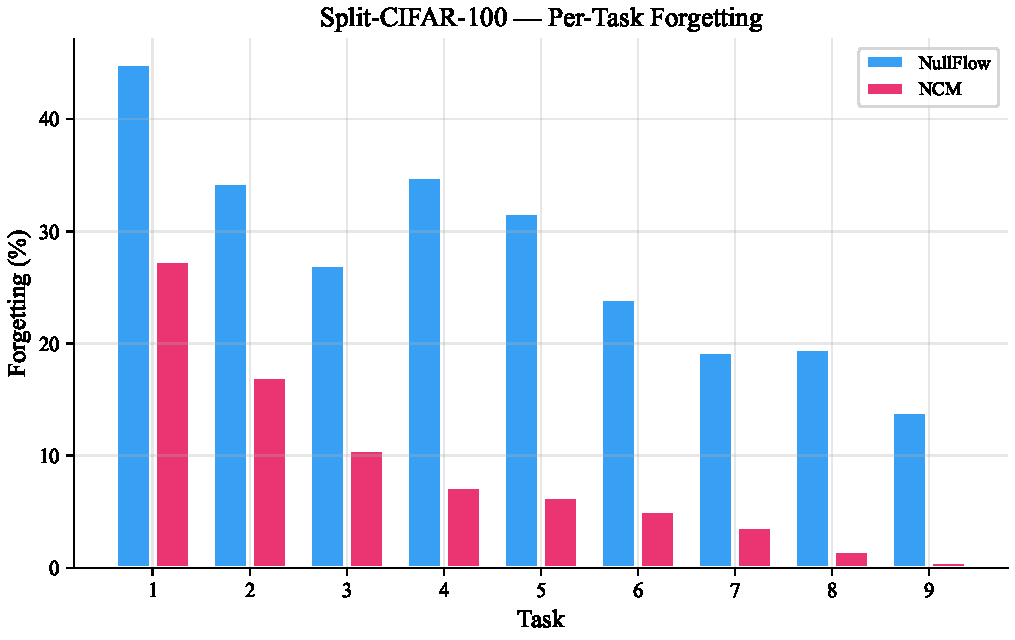
\includegraphics[width=\linewidth]{figures/cifar100/forgetting_analysis.pdf}
  \caption{Per-task forgetting analysis on Split-CIFAR-100.}
  \label{fig:forgetting}
\end{figure}

% ============================================================================
\section{Discussion}
\label{sec:discussion}
% ============================================================================

\paragraph{Context: Absolute Accuracy.}
We emphasize that all methods in our comparison operate in the same frozen ResNet-18 latent space. Recent state-of-the-art methods such as CODA-Prompt~\cite{smith2023coda} and prompt-based approaches~\cite{zhou2024revisiting} employ ViT-B/16 encoders with prompt tuning and report $>$80\% AA on Split-CIFAR-100. Our absolute numbers are lower because we deliberately use a ResNet-18 backbone, a significantly weaker encoder, to study the \textit{relative} contribution of each CL mechanism (FM, NSP, herding) in a controlled setting where all methods share identical features. The $2.65\times$ improvement over the best CL baseline (NCM) demonstrates the effectiveness of our approach \textit{independently of encoder strength}. We expect these relative gains to transfer when paired with stronger encoders.

\paragraph{On Comparing with Joint Training.}
\ours{} exceeds our Joint Training reference on both benchmarks. However, we caution against interpreting this as evidence that sequential CL surpasses the theoretical upper bound. Three asymmetries favor \ours{}: (i)~\textit{online augmentation}: \ours{} re-encodes images with fresh random crops/flips each epoch, while baselines (including Joint Training) operate on features pre-encoded once, effectively removing augmentation diversity; (ii)~\textit{training budget}: \ours{} trains the classifier for 60 epochs per task (600 total), with per-task optimizer resets and cosine scheduling, whereas Joint Training uses 100 total epochs; (iii)~\textit{regularization}: \ours{} benefits from knowledge distillation, latent noise injection, and weight alignment, which Joint Training lacks. The legitimate comparison is therefore between \ours{} and the other CL baselines, which all share the same pre-encoded features. The $2.65\times$ improvement over NCM is the core result of this work.

\paragraph{Limitations.}
\ours{} relies on a frozen ImageNet-pretrained encoder, which provides strong features for natural image benchmarks but may not generalize to domains with significant distribution shift (e.g., medical imaging, satellite imagery). The TinyImageNet results should be interpreted with the caveat that TinyImageNet is a subset of ImageNet, creating feature-level overlap in the frozen encoder. We mitigate this concern by noting that (a)~all baselines share the same encoder and thus the same potential advantage, and (b)~our CIFAR-100 results (no image-level overlap with ImageNet) confirm the same performance patterns. Additionally, the forgetting rate (28\% on CIFAR-100) remains substantial, suggesting room for improvement in knowledge preservation.

\paragraph{Computational Cost.}
The total trainable parameter count ($\sim$2.1M) is modest, and operating in latent space makes training fast ($\sim$16 minutes on Apple M1 for 10 tasks on CIFAR-100). FM replay with 6 Heun steps is $\sim$170$\times$ faster than DDPM at comparable sample quality. The entire experimental pipeline (NullFlow + 8 baselines, 3 seeds) runs on a single consumer GPU or Apple Silicon laptop.

\paragraph{Broader Impact.}
Continual learning is essential for deploying AI systems that must adapt to evolving environments. \ours{}'s efficiency and modular design (any frozen encoder + lightweight trainable modules) make it suitable for edge deployment scenarios where retraining from scratch is prohibitive.

% ============================================================================
\section{Conclusion}
\label{sec:conclusion}
% ============================================================================

We presented \ours{}, a continual learning framework that combines Conditional Flow Matching, Null-Space Projection, and herding-based exemplar management within a biologically-inspired Wake-Sleep cycle. Operating entirely in a frozen latent space, \ours{} achieves strong results on Split-CIFAR-100 (30.21$\pm$0.36\% AA, $2.65\times$ over NCM) and Split-TinyImageNet (60.77\% AA, $3.4\times$ over NCM), outperforming all CL baselines while requiring only $\sim$2.1M trainable parameters. Our ablation study confirms the complementary contributions of each component, with FM augmentation, NSP, and herding each providing significant independent gains.

Future work will explore extending \ours{} to task-free settings using Page-Hinkley drift detection, adapting the framework to non-ImageNet domains with self-supervised encoders, and investigating multi-seed evaluation on TinyImageNet for stronger statistical claims.

% ============================================================================
% References
% ============================================================================
{\small
\bibliographystyle{plain}
\begin{thebibliography}{99}

\bibitem{buzzega2020dark}
P.~Buzzega, M.~Boschini, A.~Porrello, D.~Davoli, and S.~Calderara.
\newblock Dark experience for general continual learning: a strong, simple baseline.
\newblock In \textit{NeurIPS}, 2020.

\bibitem{chaudhry2019tiny}
A.~Chaudhry, M.~Ranzato, M.~Rohrbach, and M.~Elhoseiny.
\newblock Efficient lifelong learning with {A-GEM}.
\newblock In \textit{ICLR}, 2019.

\bibitem{deng2009imagenet}
J.~Deng, W.~Dong, R.~Socher, L.-J.~Li, K.~Li, and L.~Fei-Fei.
\newblock Image{N}et: A large-scale hierarchical image database.
\newblock In \textit{CVPR}, 2009.

\bibitem{french1999catastrophic}
R.~M. French.
\newblock Catastrophic forgetting in connectionist networks.
\newblock \textit{Trends in Cognitive Sciences}, 3(4):128--135, 1999.

\bibitem{he2016deep}
K.~He, X.~Zhang, S.~Ren, and J.~Sun.
\newblock Deep residual learning for image recognition.
\newblock In \textit{CVPR}, 2016.

\bibitem{hinton1995wake}
G.~E. Hinton, P.~Dayan, B.~J. Frey, and R.~M. Neal.
\newblock The ``wake-sleep'' algorithm for unsupervised neural networks.
\newblock \textit{Science}, 268(5214):1158--1161, 1995.

\bibitem{janson2022simple}
S.~Janson, Y.~Zhang, and A.~Sugiyama.
\newblock A simple baseline that questions the use of pretrained-models in continual learning.
\newblock In \textit{NeurIPS Workshop on Distribution Shifts}, 2022.

\bibitem{kirkpatrick2017overcoming}
J.~Kirkpatrick, R.~Pascanu, N.~Rabinowitz, J.~Veres, G.~Desjardins, A.~A. Rusu, K.~Milan, J.~Quan, T.~Ramalho, A.~Grabska-Barwinska, et~al.
\newblock Overcoming catastrophic forgetting in neural networks.
\newblock \textit{PNAS}, 114(13):3521--3526, 2017.

\bibitem{krizhevsky2009learning}
A.~Krizhevsky.
\newblock Learning multiple layers of features from tiny images.
\newblock Technical report, University of Toronto, 2009.

\bibitem{kumaran2016learning}
D.~Kumaran, D.~Hassabis, and J.~L. McClelland.
\newblock What learning systems do intelligent agents need? {C}omplementary learning systems theory updated.
\newblock \textit{Trends in Cognitive Sciences}, 20(7):512--534, 2016.

\bibitem{li2017learning}
Z.~Li and D.~Hoiem.
\newblock Learning without forgetting.
\newblock \textit{IEEE TPAMI}, 40(12):2935--2947, 2017.

\bibitem{lipman2023flow}
Y.~Lipman, R.~T.~Q. Chen, H.~Ben-Hamu, M.~Nickel, and M.~Le.
\newblock Flow matching for generative modeling.
\newblock In \textit{ICLR}, 2023.

\bibitem{liu2022flow}
X.~Liu, C.~Gong, and Q.~Liu.
\newblock Flow straight and fast: Learning to generate and transfer data with rectified flow.
\newblock In \textit{ICLR}, 2023.

\bibitem{mallya2018packnet}
A.~Mallya and S.~Lazebnik.
\newblock {PackNet}: Adding multiple tasks to a single network by iterative pruning.
\newblock In \textit{CVPR}, 2018.

\bibitem{mccloskey1989catastrophic}
M.~McCloskey and N.~J. Cohen.
\newblock Catastrophic interference in connectionist networks: The sequential learning problem.
\newblock \textit{Psychology of Learning and Motivation}, 24:109--165, 1989.

\bibitem{prabhu2020gdumb}
A.~Prabhu, P.~Torr, and P.~Dokania.
\newblock {GDumb}: A simple approach that questions our progress in continual learning.
\newblock In \textit{ECCV}, 2020.

\bibitem{rebuffi2017icarl}
S.-A.~Rebuffi, A.~Kolesnikov, G.~Sperl, and C.~H. Lampert.
\newblock i{C}a{RL}: Incremental classifier and representation learning.
\newblock In \textit{CVPR}, 2017.

\bibitem{rusu2016progressive}
A.~A. Rusu, N.~C. Rabinowitz, G.~Desjardins, H.~Sober, K.~Kavukcuoglu, and R.~Hadsell.
\newblock Progressive neural networks.
\newblock \textit{arXiv preprint arXiv:1606.04671}, 2016.

\bibitem{saha2021gradient}
G.~Saha, I.~Garg, and K.~Roy.
\newblock Gradient projection memory for continual learning.
\newblock In \textit{ICLR}, 2021.

\bibitem{shin2017continual}
H.~Shin, J.~K. Lee, J.~Kim, and J.~Kim.
\newblock Continual learning with deep generative replay.
\newblock In \textit{NeurIPS}, 2017.

\bibitem{welling2009herding}
M.~Welling.
\newblock Herding dynamical weights to learn.
\newblock In \textit{ICML}, 2009.

\bibitem{zeng2019continual}
G.~Zeng, Y.~Chen, B.~Cui, and S.~Yu.
\newblock Continual learning of context-dependent processing in neural networks.
\newblock \textit{Nature Machine Intelligence}, 1(8):364--372, 2019.

\bibitem{zenke2017continual}
F.~Zenke, B.~Poole, and S.~Ganguli.
\newblock Continual learning through synaptic intelligence.
\newblock In \textit{ICML}, 2017.

\bibitem{zhao2020maintaining}
B.~Zhao, X.~Xiao, G.~Gan, B.~Zhang, and S.-T. Xia.
\newblock Maintaining discrimination and fairness in class incremental learning.
\newblock In \textit{CVPR}, 2020.

\bibitem{zhou2024revisiting}
D.-W.~Zhou, H.-J.~Ye, D.-C.~Zhan, and Z.~Liu.
\newblock Revisiting class-incremental learning with pre-trained models: Generalizability and adaptivity are all you need.
\newblock \textit{IJCV}, 2024.

\bibitem{smith2023coda}
J.~S. Smith, L.~Karlinsky, V.~Gutta, P.~Cascante-Bonilla, D.~Kim, A.~Arbelle, R.~Panda, R.~Feris, and Z.~Kira.
\newblock {CODA-Prompt}: {CO}ntinual decomposed attention-based prompting for rehearsal-free continual learning.
\newblock In \textit{CVPR}, 2023.

\bibitem{van2020brain}
G.~M. van~de~Ven, H.~T. Siegelmann, and A.~S. Tolias.
\newblock Brain-inspired replay for continual learning with artificial neural networks.
\newblock \textit{Nature Communications}, 11(1):4069, 2020.

\end{thebibliography}
}

\end{document}
